\documentclass[12pt,a4paper]{article}

\usepackage{comment}
\usepackage[english]{babel}
\usepackage[utf8]{inputenc}
\usepackage{amsmath}
\usepackage{amssymb}
\usepackage{graphicx}
\usepackage{hyperref}
\usepackage{todonotes}
\setuptodonotes{inline}

\begin{document}
\thispagestyle{empty}
\begin{center}
Rheinisch-Westf\"alische Technische Hochschule Aachen \\
Alessandro Berti\\[6ex]

\LARGE
\textbf{Evaluation: Does conformance information derived from a process model improve the prediction of future deviations and compliance risks?} \\[6ex]
        \centering{Group 4:}\\
	\textit{Richard Schuppener, Cem Colak} \\[6ex]
\end{center}

\newpage

\tableofcontents
\newpage

\section{Introduction}
In the following we will evaluate two different experimental studies - based on the full(Experimental study 2) and filtered (Experimental study 1) event log \textit{Sepsis Cases} - to compare and evaluate the usage of conformance information in the predictions of future deviations and compliance risks. Later, we will discuss the overall viability of the usage of conformance information in predictive process mining tasks.

In the event log \textit{Sepsis Cases}, cases represent patients going through a sepsis-specific handling pathway in a hospital. The data is anonymized and timestamps have been randomized. Events were recorded using an ERP. Additionally, 39 case attributes are present in the log.

\section{Experimental Study 1: Remaining Time Prediction of Sepsis cases}
As an experimental study, we want to predict the remaining time of specific prefix lengths. In application, remaining time plays a huge role in time-bounded cases. In hospital's e.g. sepsis-diagnosis for example, remaining time is specifically important since the severity of the disease could worsen or even lead to unlucky outcomes. Therefore, having a remaining time prediction(optimally connected to specific activities), can be used to build an early-warn-system and recommendations for later activities such that the remaining time of a diagnosis can actively be lowered.
In this experimental study we have used a filtered version of the sepsis cases, where we filtered out all the cases having a higher duration of approximately 30 days. We did it for simplicity reasons, such that we have a more homogenous event log. This is due to the huge variations in its case durations: Some cases have a duration of over one year, wheras others have a duration of around one day.

In real-life application, this approach is not recommended, since the remaining time prediction's outcomes target are explicitly those cases, which have a duration exceeding specific thresholds.

In the following evaluation, I will focus on multiple variations of algorithms with their respective parameters. However, most of the chosen parameters of the CLI walkthroughs remain the same. Furthermore, the discovered Petri net visualization itself carries no meaning for the remaining-time target, so we neither display nor save it. However, a process model still has to be \emph{discovered} so that the alignment-based (conformance-aware) features can be computed for the conformance-based runs.
For all the following outcomes, we configured the following standard parameters:

\begin{enumerate}
	\item Prediction Target: ``Remaining time''
	\item Prefix Mode: varying, 1 to 8
	\item Split value: 0.7
	\item Discovery algorithm (for the alignment features): Inductive miner with noise threshold 0.2 % [assumption --- please proofread / adjust]
\end{enumerate}

With these settings, we compare three regression algorithms, each trained once on the control flow (base model) and once on control flow augmented with alignments (conformance-based):
\begin{enumerate}
	\item Decision Tree Regressor
	\begin{enumerate}
		\item \texttt{max\_depth}: 8
		\item \texttt{random\_state}: 42
	\end{enumerate}
	\item Random Forest Regressor
	\begin{enumerate}
		\item \texttt{n\_estimators}: 100
		\item \texttt{random\_state}: 42
	\end{enumerate}
	\item Gradient Boosting Regressor
	\begin{enumerate}
		\item \texttt{random\_state}: 42
	\end{enumerate}
\end{enumerate}

Additionally, our regression pipeline outputs the root mean squared error (RMSE) and the mean absolute error (MAE). In this study we report \emph{only} the MAE, because it simply averages the absolute values of the deviations, making it an appropriate metric to explain to non-technical stakeholders. All errors are reported in \emph{days} (the CLI automatically selects a human-readable time unit).


\subsection{Evaluation protocol}
The filtered log of $844$ cases is split $0.7\,/\,0.3$ into training and test \emph{cases} before any prefix extraction, so that no prefix of a test case can leak into the training data. Each case is then expanded into all prefixes of length $1$ to $8$, yielding $4476$ training and $1824$ test prefix-instances. The label of a prefix is the true remaining time (in seconds) from the end of that prefix to the completion of its case.

\subsection{Results}
Table~\ref{tab:rt_mae} reports the global MAE (pooled over prefix lengths $1$--$8$) for every regressor and feature set.

\begin{table}[htbp]
	\centering
	\begin{tabular}{l c c}
		\hline
		\textbf{Regressor} & \textbf{Control-flow (base)} & \textbf{conformance-aware} \\
		\hline
		Decision Tree     & $5.17$ & $5.35$ \\
		Random Forest     & $5.46$ & $5.27$ \\
		Gradient Boosting & $\mathbf{4.98}$ & $5.00$ \\
		\hline
	\end{tabular}
	\caption{Global Mean Absolute Error (in days) by regressor and feature set, pooled over prefix lengths $1$--$8$. Lower is better; the best value is shown in bold.}
	\label{tab:rt_mae}
\end{table}

Two patterns stand out. First, \textbf{Gradient Boosting} is the strongest regressor in both feature sets ($\approx 5.0$ days), whereas the Random Forest is the weakest on the control-flow features. Second, and more important for our research question, \textbf{adding conformance (alignment) information does not improve the remaining-time prediction}: the conformance-aware MAE is essentially equal to (Gradient Boosting: $5.00$ vs.\ $4.98$ days) or slightly worse than (Decision Tree) the control-flow baseline, and only the Random Forest shows a marginal gain for the conformance-aware case. This mirrors the conclusion of Experimental Study~2.
Figure~\ref{fig:rt_mae_by_len} shows the MAE as a function of prefix length for all six configurations.

\begin{figure}[htbp]
	\centering
	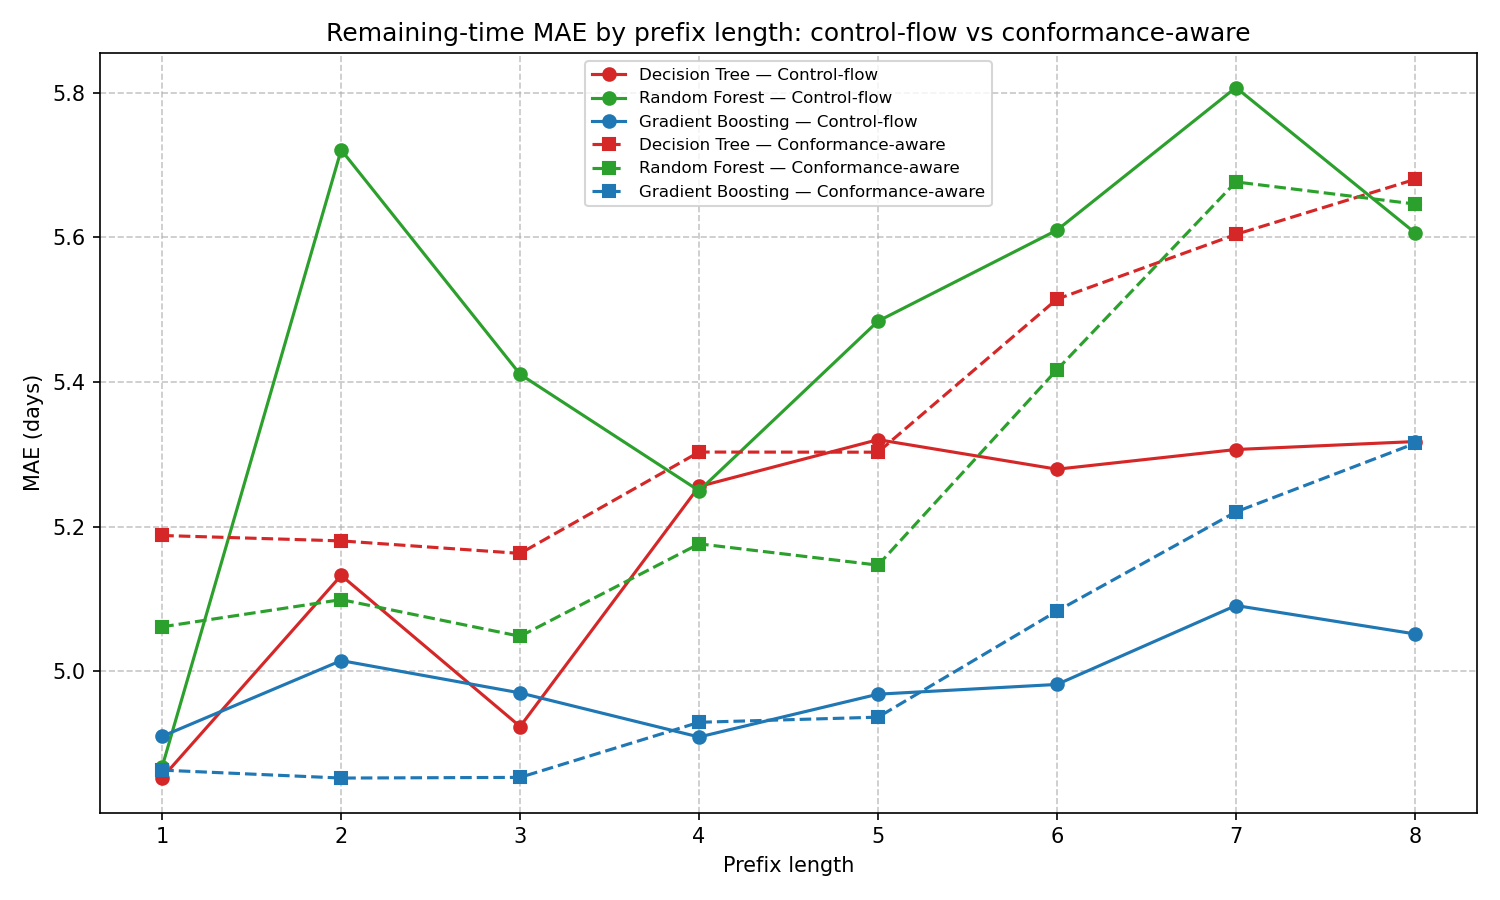
\includegraphics[width=0.9\textwidth]{figures/sepsis_remaining_time/mae_by_prefix_comparison.png}
	\caption{Remaining-time MAE (days) by prefix length for the three regressors on control-flow (solid lines) vs.\ conformance-aware (dashed lines) features.}
	\label{fig:rt_mae_by_len}
\end{figure}

Contrary to the intuition that observing more of a case should make its remaining time easier to predict, the MAE stays flat or even drifts slightly \emph{upward} as the prefix grows from $1$ to $8$ (e.g.\ Gradient Boosting on control-flow rises from $\approx 4.9$ to $\approx 5.1$ days). The Gradient Boosting curves sit lowest and are the most stable, while the Random Forest curves are the highest and most volatile. For every regressor the control-flow and conformance-aware curves track each other closely, again indicating that the alignment features add little signal. The number of test instances per length decreases ($242 \to 200$) as the shorter cases run out of events.

To understand the error structure, Figure~\ref{fig:rt_diag} shows the predicted-vs-actual scatter (left) and the residual distribution (right) for the best model (Gradient Boosting on control-flow features).

\begin{figure}[htbp]
	\centering
	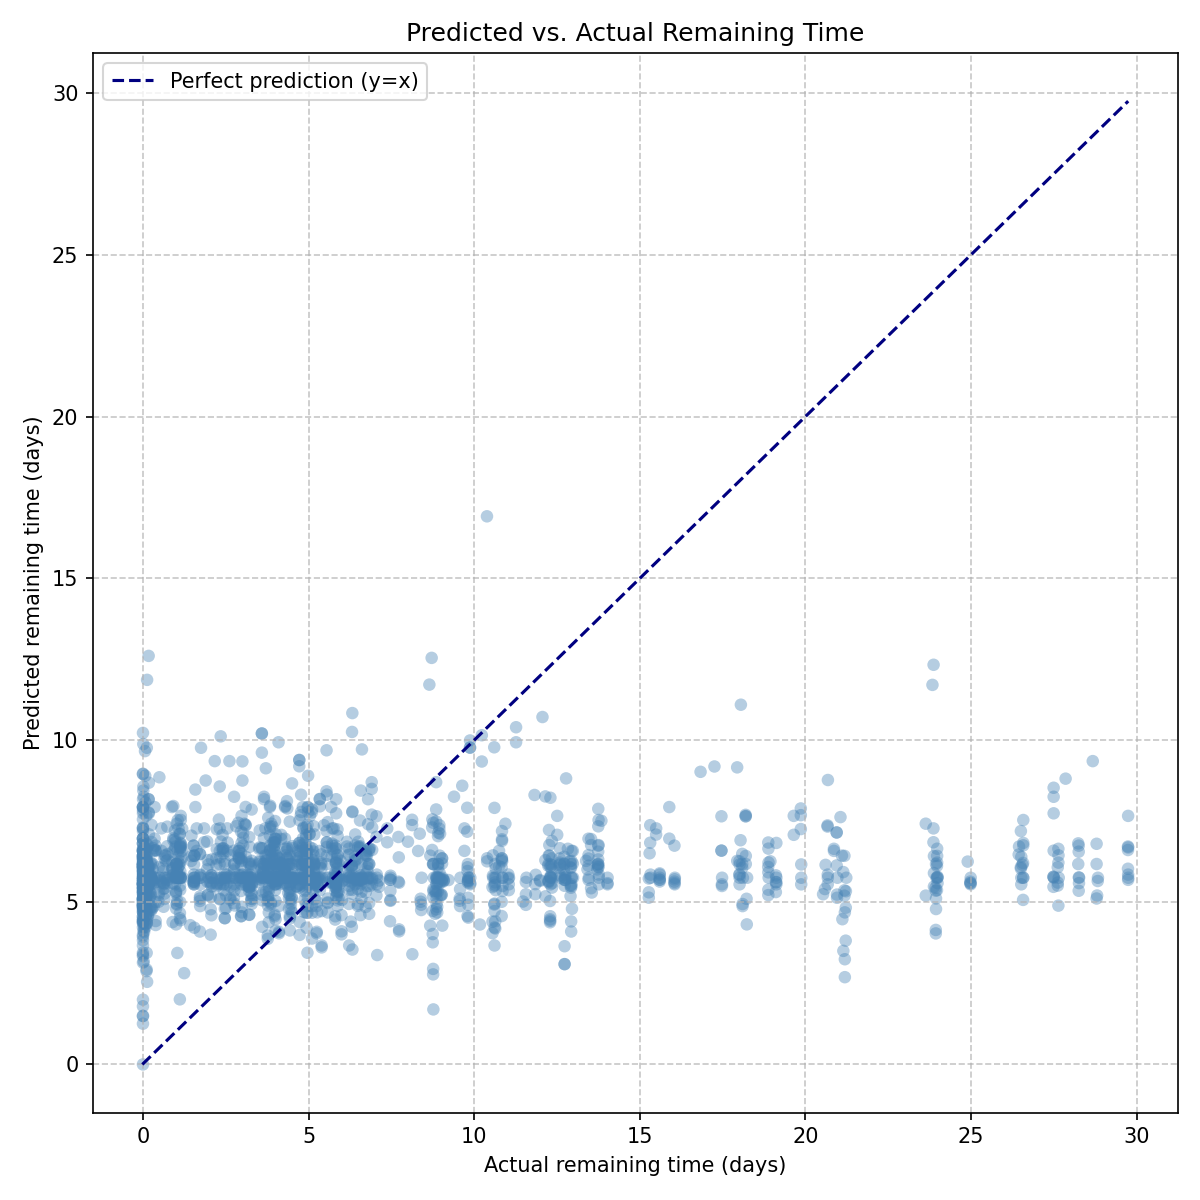
\includegraphics[width=0.48\textwidth]{figures/sepsis_remaining_time/control_flow_gradient_boosting_predicted_vs_actual.png}
	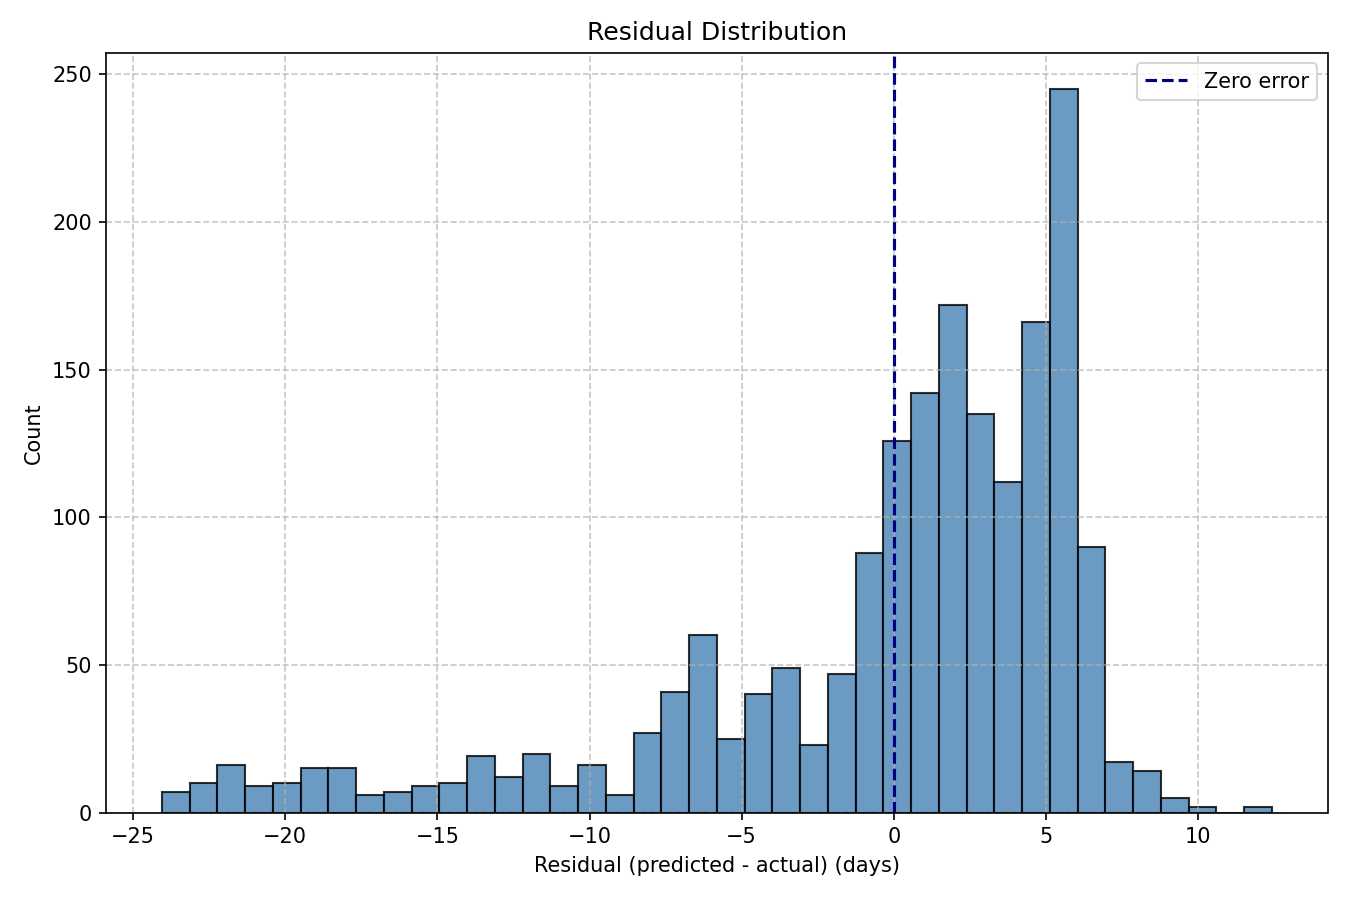
\includegraphics[width=0.48\textwidth]{figures/sepsis_remaining_time/control_flow_gradient_boosting_residuals.png}
	\caption{Predicted vs.\ actual remaining time (left) and residual distribution (right) for the Gradient Boosting regressor on control-flow features.}
	\label{fig:rt_diag}
\end{figure}

The scatter plot reveals the core limitation: the model compresses almost all predictions into a narrow band of roughly $3$--$7$ days regardless of the true remaining time. Cases with a large actual remaining time ($10$--$30$ days) are therefore strongly \emph{under}-predicted (points far below the $y=x$ line), a classic regression-to-the-mean effect. The residual histogram confirms this: most residuals sit slightly above zero (the many near-completion prefixes are over-predicted by a few days), but a heavy left tail reaches down to $-25$ days from the minority of long-running cases. This asymmetry is the main driver of the $\approx 5$-day MAE, and it is a property of the (filtered) data rather than of the feature set --- which is precisely why the conformance features cannot help.

\subsection{Computational aspects}
The conformance-aware pipeline is markedly more expensive. On the same split, control-flow feature extraction over prefixes $1$--$8$ took $\approx 0.2$\,s and produced $16$ features, whereas the conformance-aware extraction took $\approx 4.4$\,s --- about $20\times$ longer, dominated by alignment computation --- and produced $165$ features. Training times were small throughout ($\le 3.5$\,s per regressor). Crucially, this extra cost did \emph{not} translate into a lower MAE. Because alignments are recomputed for every prefix, the cost grows with prefix length and, more steeply, with log size; on larger or unfiltered logs (the full Sepsis log, or the BPI Challenge logs) alignment computation becomes the dominant and fastest-growing cost, so the conformance-aware approach scales poorly relative to its (here, absent) predictive benefit.

\subsection{Threats to validity and Future work}
This experimental study showed, that control-flow-based models exhibit a stronger overall outcome for this specific configuration and event log. Nevertheless, it is highly narrowed to specific parameters mirroring our observations on the overall validity of the usage of conformance-based diagnostics. Opposed to our observations, we think that alignments can still improve predicion pipelines, but requires further investigation into the algorithms and features used for prediction.

\section{Experimental study 2: Process Outcome of Sepsis Cases}
A suitable application would be to predict the outcome of a case. Since there is a set of different discharge types - as they are called in a study on patient trajectories \cite{sepsis_study} - \textit{Release A-E}, we can easily set these as the \texttt{Process Outcome} prediction type in our CLI. Note, that \textit{uncertain outcome} signifies, that none of these discharges were executed in the given case. To do so, we need to select \texttt{Process Outcome} as prediction goal and specify the activity names that represent the outcomes.
In the following, we will present results based on:
\begin{enumerate}
        \item Control-flow only (base model)
        \item Case-attributes only
        \item Control-flow and alignments (conformance aware)
        \item Different prefix lengths (only relevant for control-flow and alignments)
\end{enumerate}
\subsection{Control-flow only}
\begin{itemize}
        \item Discovery algorithm: Inductive miner with noise threshold $0.2$
        \item Prediction target: Process outcome with outcome activties \textit{Release A-E}
        \item Classification algorithm: Gradient Boosting / Logistic Regression with standard hyper-parameters
\end{itemize}
We observe that the model predicts primarily the majority labels (such as \textit{Release A} and \textit{uncertain\_outcome}). For prefix length 6 and prefix length 13 (median), the confusion matrices and per-class accuracies are displayed in Figures \ref{fig:control_flow_confusion_matrices} and \ref{fig:control_flow_per_class_accuracies}. This might be due to the fact, that \textit{Release A} contributes to 63.6\% and in 25.8\%, the discharge activity is skipped.

The model achieves high accuracy on the majority class \textit{Release A} (around 97\%) and the \textit{uncertain\_outcome} class (around 87-89\%), but performs poorly on the minority outcomes (\textit{Release B-E}), which are rarely predicted correctly due to the class imbalance.

\begin{figure}[htbp]
	\centering
	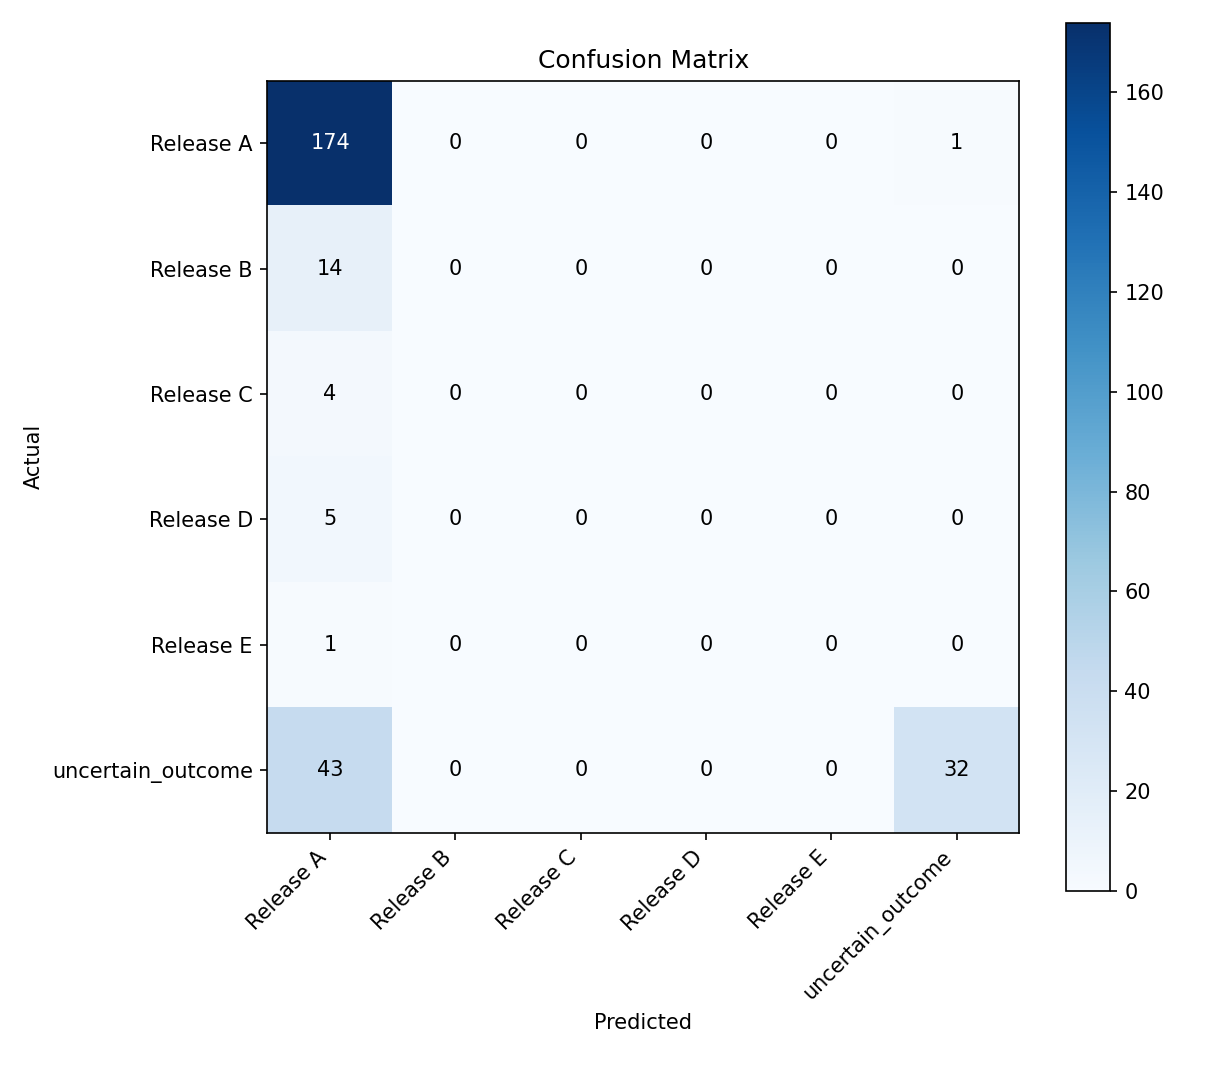
\includegraphics[width=0.48\textwidth]{figures/sepsis/control_flow_confusion_matrix_len6.png}
	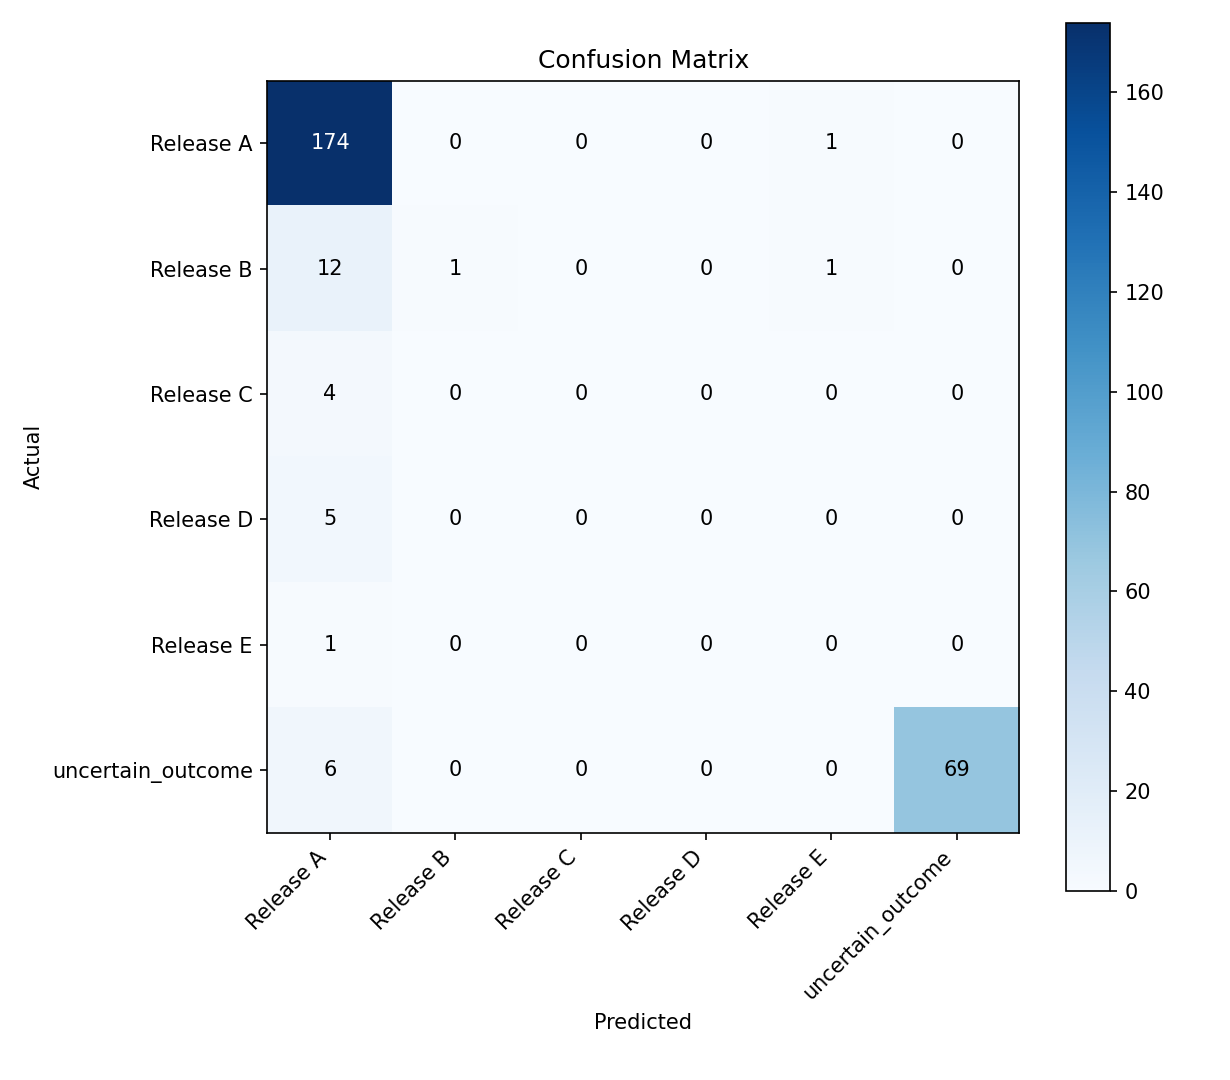
\includegraphics[width=0.48\textwidth]{figures/sepsis/control_flow_confusion_matrix_len13.png}
	\caption{Confusion matrices for prefix length 9 (left) and 13 (right) for control-flow only classifier.}
	\label{fig:control_flow_confusion_matrices}
\end{figure}

\begin{figure}[htbp]
	\centering
	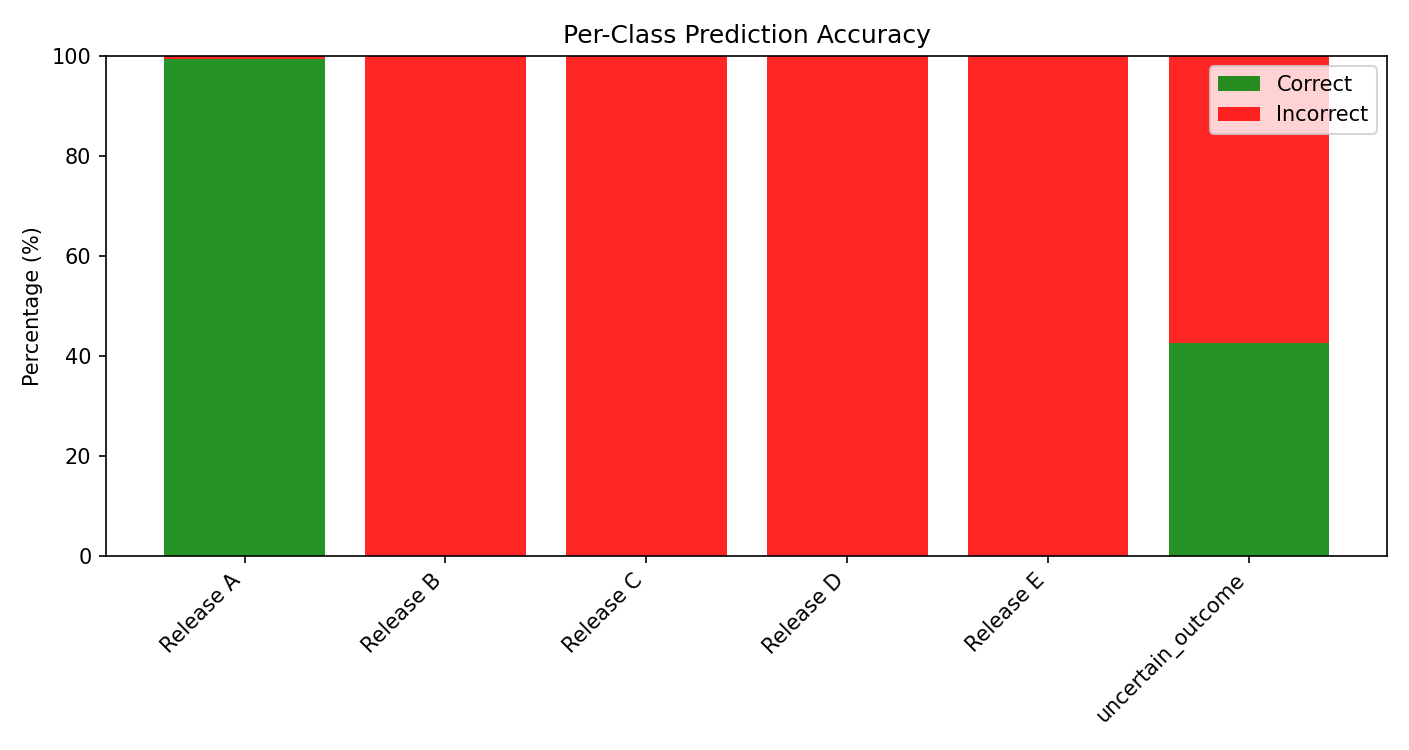
\includegraphics[width=0.48\textwidth]{figures/sepsis/control_flow_per_class_accuracy_len6.png}
	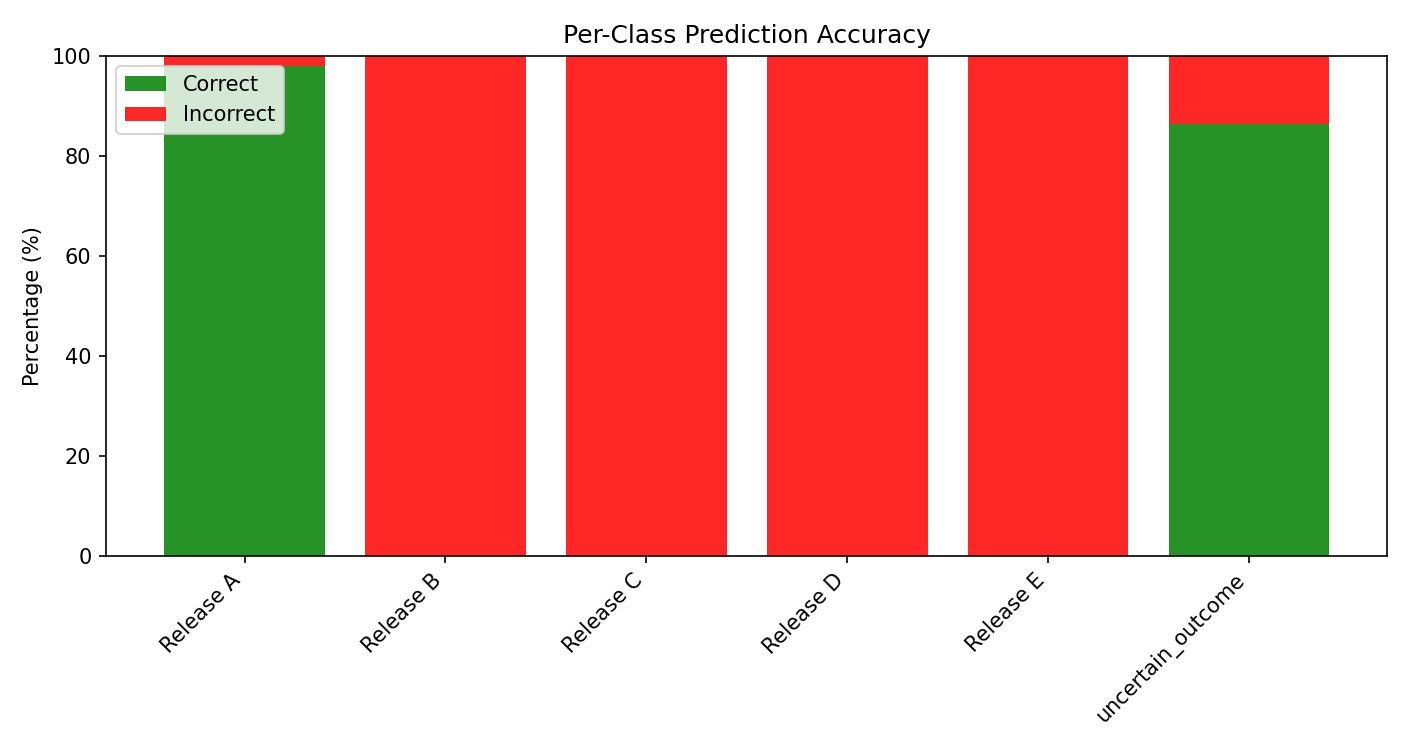
\includegraphics[width=0.48\textwidth]{figures/sepsis/control_flow_per_class_accuracy_len13.png}
	\caption{Per-class accuracies for prefix length 6 (left) and 13 (right) for control-flow only classifier.}
	\label{fig:control_flow_per_class_accuracies}
\end{figure}

Naturally, we are interested in the question
\begin{quotation}
\textit{What influence does the length of the prefixes have on the prediction quality (e.g. accuracy, F1)?}
\end{quotation}
To answer this, we visualize the accuracy and F1-score per prefix length in \ref{fig:control_flow_by_len_vis}. As the prefix length increases from 1 to 15, the accuracy increases from approximately 0.63 to 0.81, and the F1 score increases from 0.48 to 0.78.
\begin{figure}[t]
	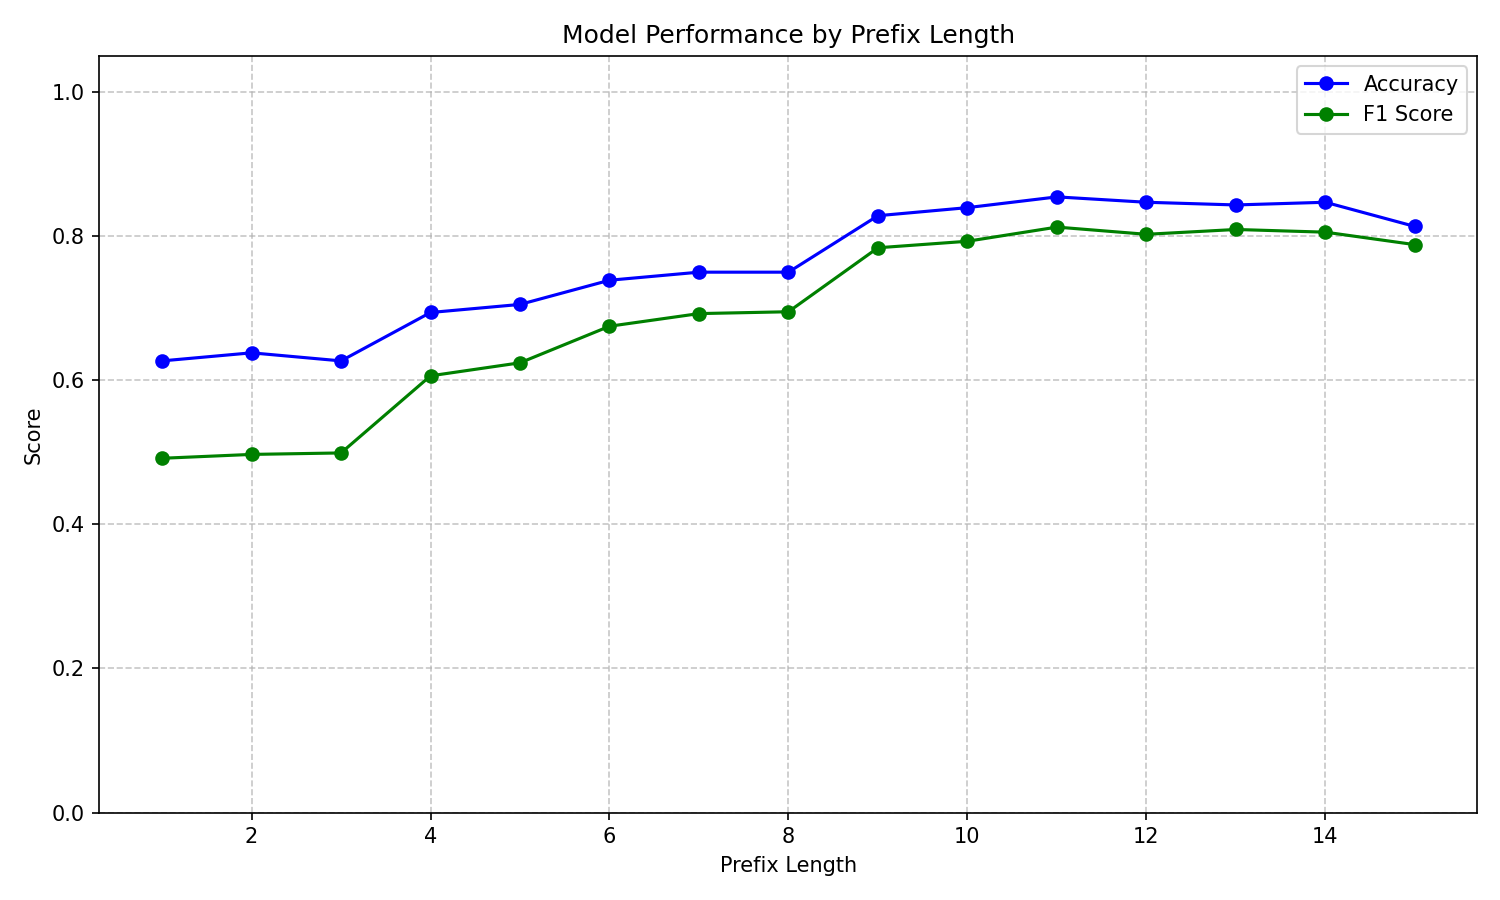
\includegraphics[width=1\textwidth]{figures/sepsis/control_flow_by_len_vis.png}
	\caption{Accuracy and F1 score based on prefix length for control-flow only classifier.}
	\label{fig:control_flow_by_len_vis}
\end{figure}

We can also visualize the importance of the given features. The most important features are the occurrences of clinical activities like \textit{Admission NC} (Normal Care admission), \textit{Admission IC} (Intensive Care admission), \textit{IV Liquid}, and \textit{IV Antibiotics}. Figure \ref{fig:control_flow_feature_importances} shows the top predictive features for both prefix lengths. It can be clearly observed, that the feature importance does change depending on the prefix length.

\begin{figure}[htbp]
	\centering
	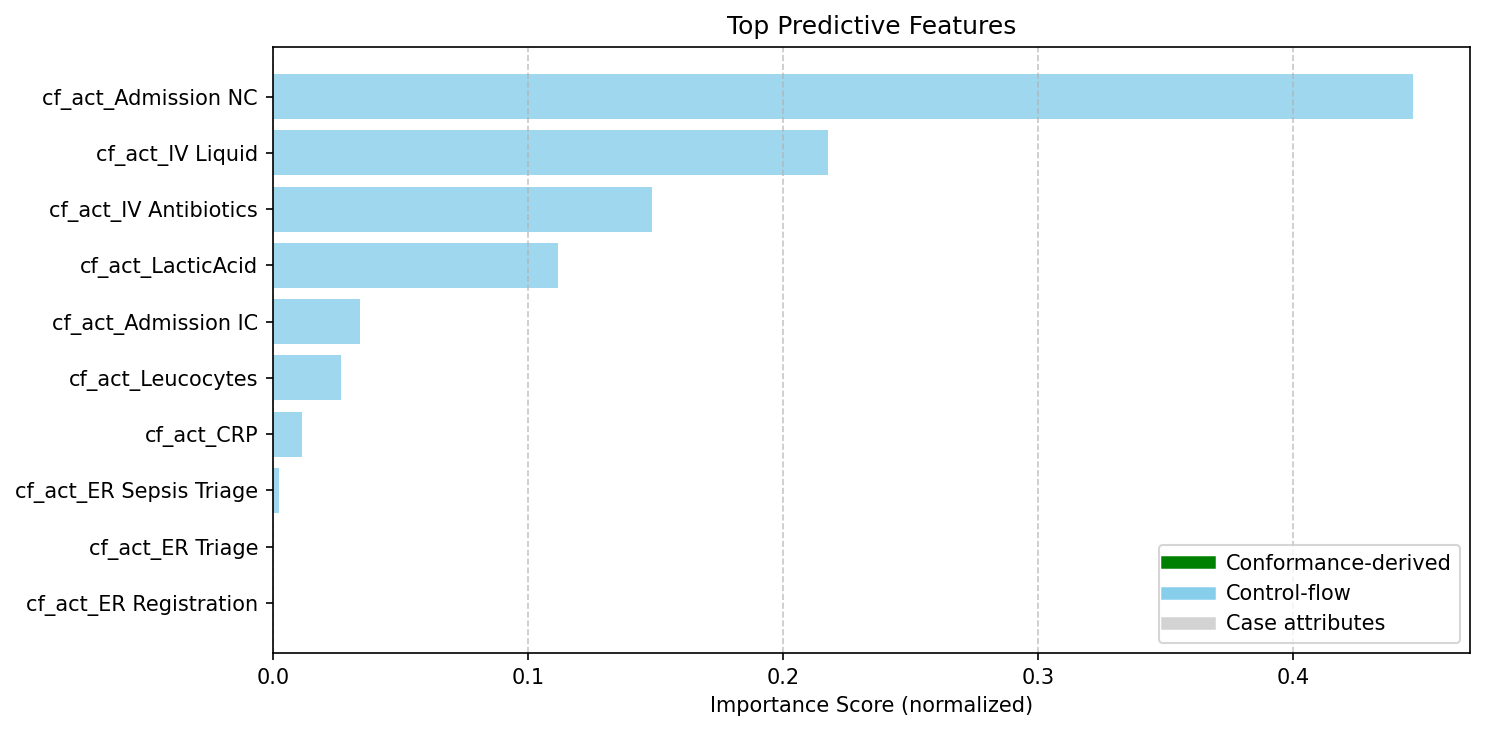
\includegraphics[width=0.48\textwidth]{figures/sepsis/control_flow_feature_importance_len6.png}
	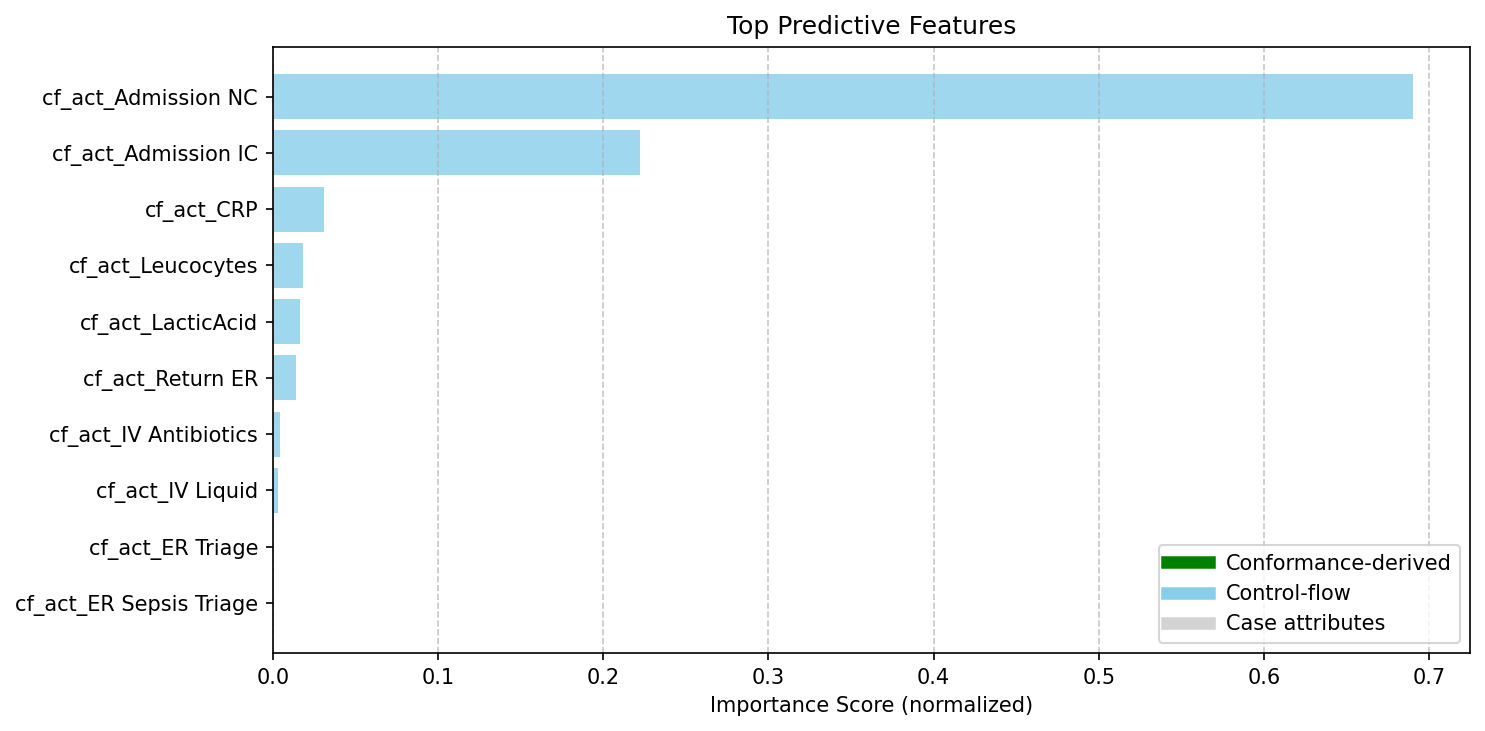
\includegraphics[width=0.48\textwidth]{figures/sepsis/control_flow_feature_importance_len13.png}
	\caption{Importance of features for prefix length 6 (left) and 13 (right) for control-flow only classifier.}
	\label{fig:control_flow_feature_importances}
\end{figure}
Subsequently, we will analyze the resource consumption by our code by dissecting the total time into the time spent on specific pipeline steps, as well as stating the peak memory consumed during the execution. The runtime of our code is depicted in \ref{fig:control_flow_runtime}. It shows us that the majority of time is consumed by the discovery and the model training - this is to be expected.
\begin{figure}[htbp]
	\centering
	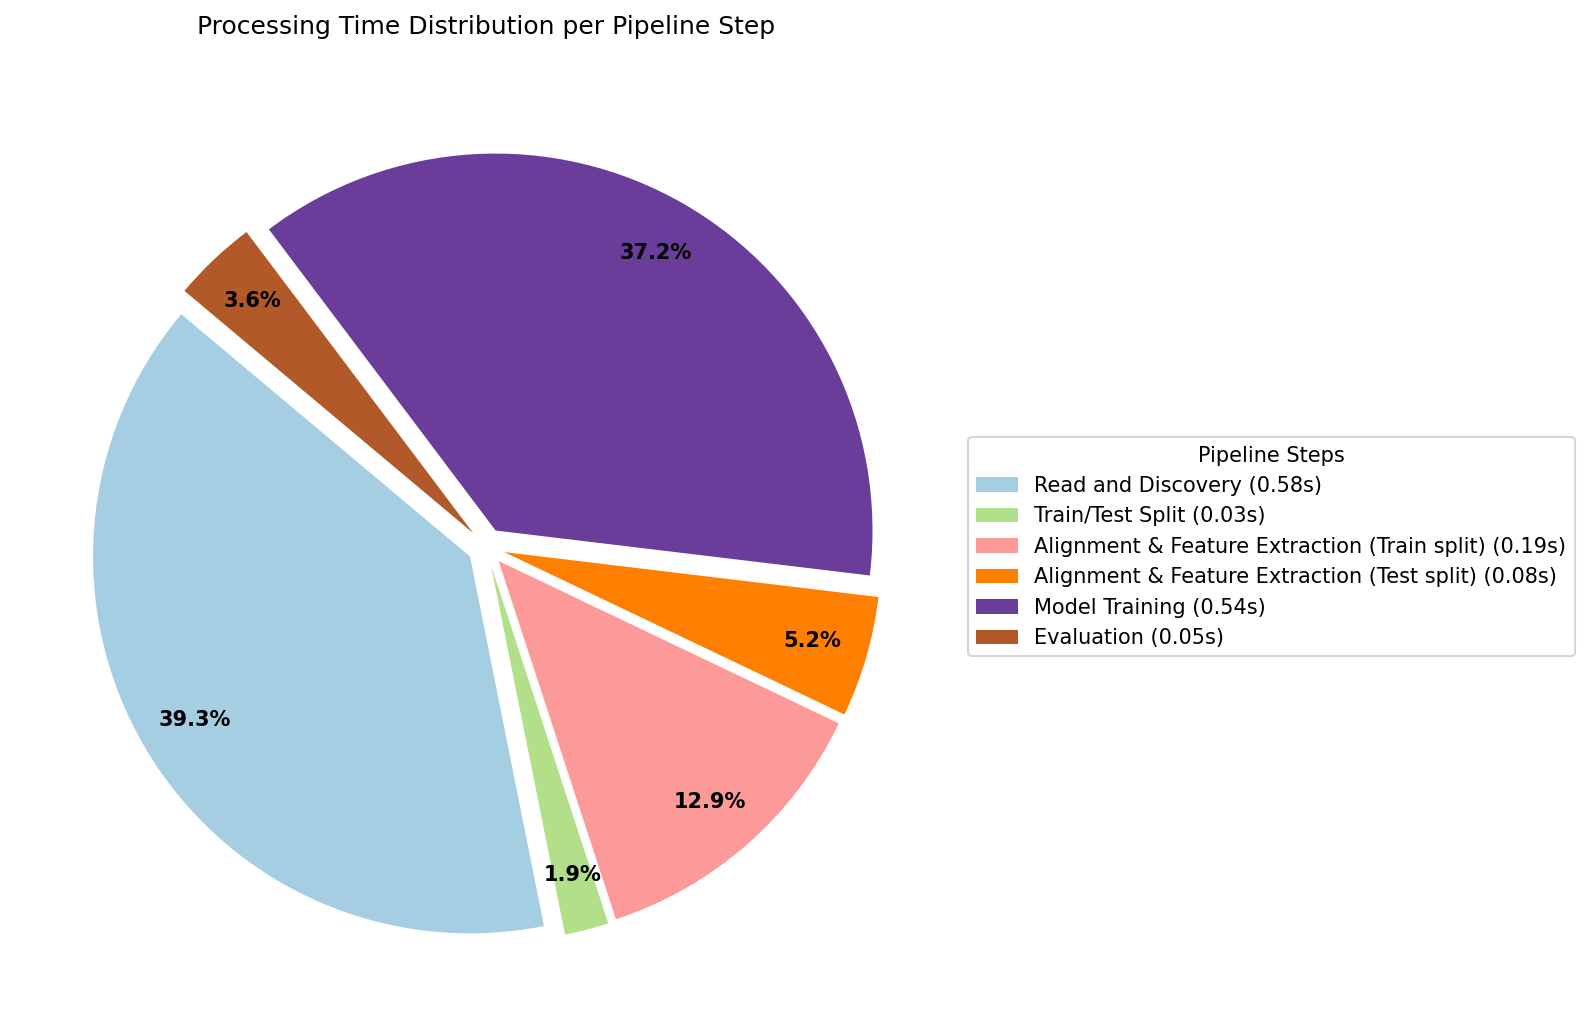
\includegraphics[width=1\textwidth]{figures/sepsis/control_flow_runtime.png}
	\caption{Runtime of the control-flow based classifier.}
	\label{fig:control_flow_runtime}
\end{figure}

\subsection{Case attributes only}
For the case-attributes-only approach, we utilize the static trace-level attributes (such as age, clinical criteria, and diagnosis codes) associated with each patient's case. Since these attributes are static and do not change as the case progresses, the prefix length is irrelevant for this model. We split the event log (75\% training, 25\% testing) and train a Logistic Regression classifier on all available case attributes to predict the discharge types.

The model achieves an overall accuracy of 81\% and an F1-score of 78\%. As shown in the confusion matrix and the per-class accuracy bar chart (Figure \ref{fig:case_attributes_eval}), the classifier performs moderately well on the majority outcome \textit{Release A} (89.9\% correct) and achieves high success on the \textit{uncertain\_outcome} class (93.3\% correct). However, due to class imbalance and the static nature of the attributes, prediction accuracy for minority discharge outcomes (\textit{Release B-E}) remains extremely low.

\begin{figure}[htbp]
	\centering
	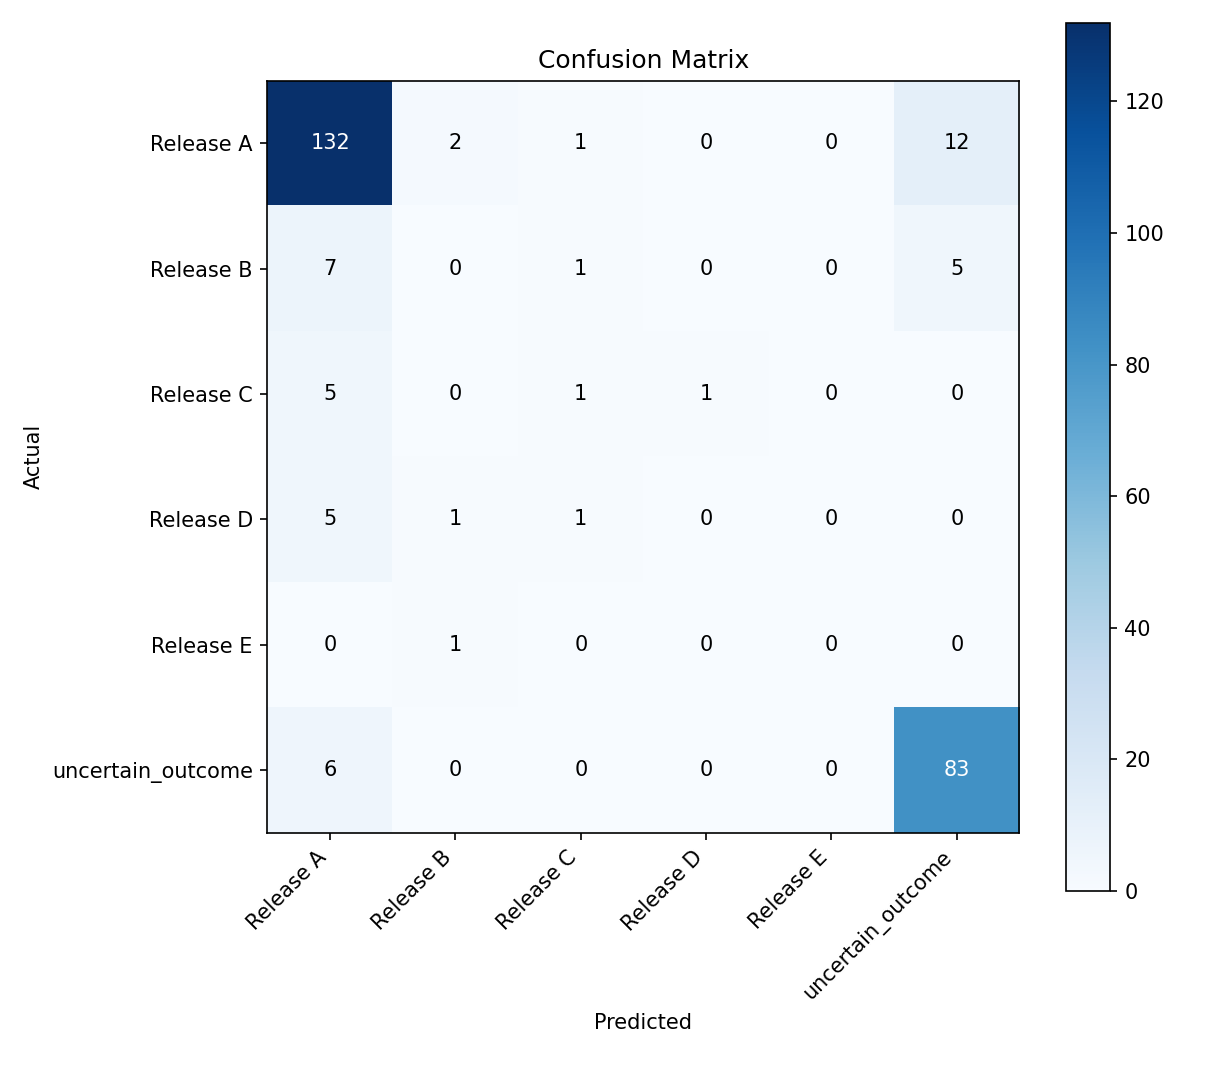
\includegraphics[width=0.48\textwidth]{figures/sepsis/case_attributes_confusion_matrix.png}
	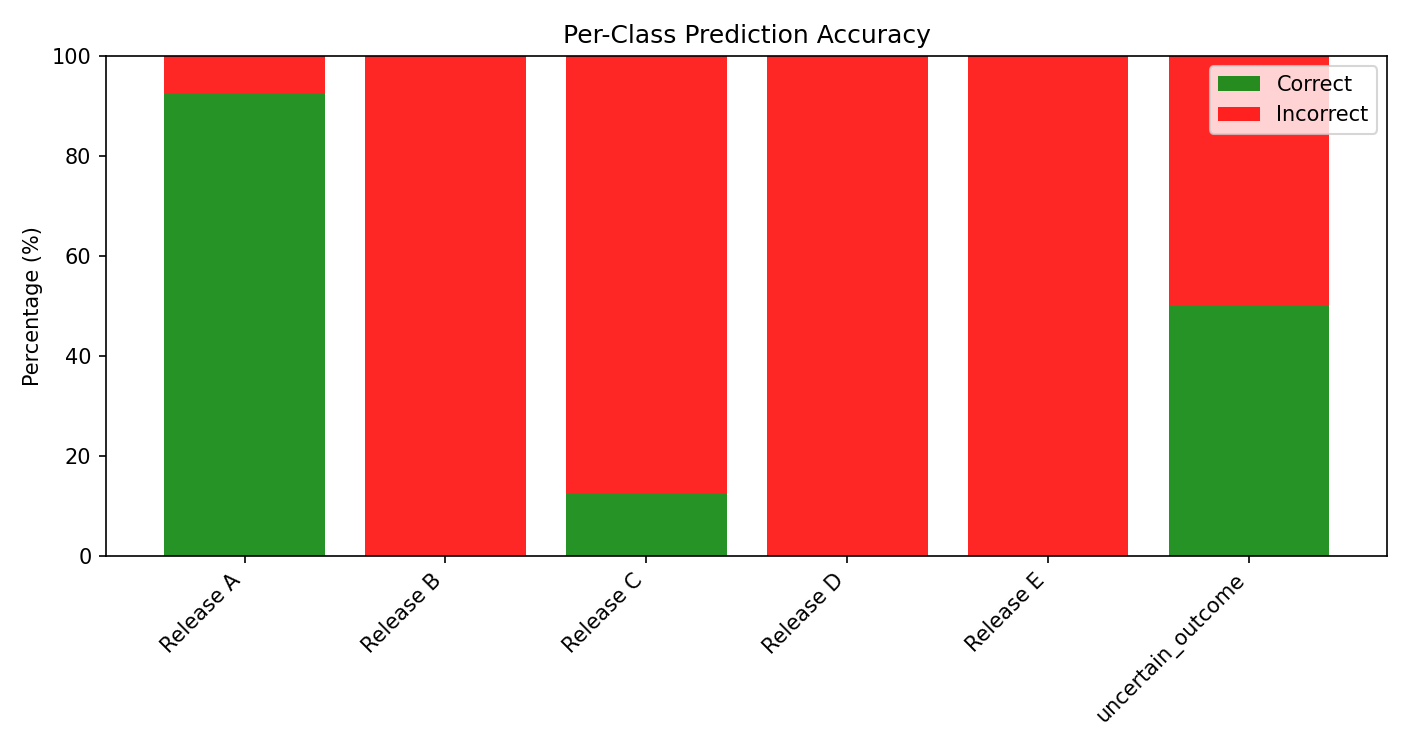
\includegraphics[width=0.48\textwidth]{figures/sepsis/case_attributes_per_class_accuracy.png}
	\caption{Confusion matrix (left) and per-class accuracies (right) for the case-attributes-only classifier.}
	\label{fig:case_attributes_eval}
\end{figure}

The feature importance chart (Figure \ref{fig:case_attributes_feature_importance}) shows the top predictive attributes. Here, it seems that many attributes are similarly predictive. This might be attributed to correlation or causation between the case attributes.

\begin{figure}[htbp]
	\centering
	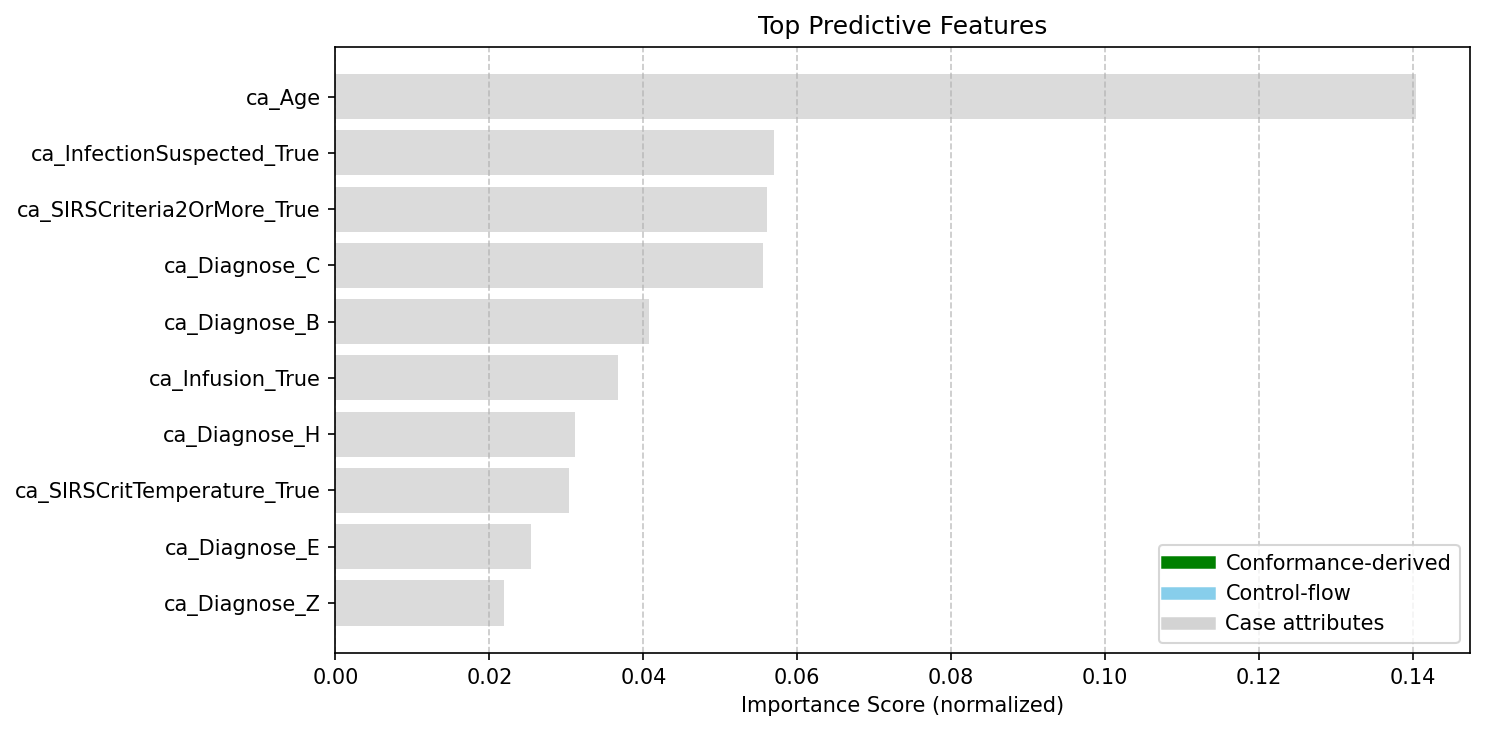
\includegraphics[width=0.7\textwidth]{figures/sepsis/case_attributes_feature_importance.png}
	\caption{Feature importances for the case-attributes-only classifier.}
	\label{fig:case_attributes_feature_importance}
\end{figure}

\subsection{Alignment-based}
Another way to gain more information about a case is to align the trace to the process model. Using the inductive miner with a noise threshold of 0.2, we discovered a normative process model with which we can determine traces deviating from the discovered to-be process execution. Of course, it must be noted that this does not provide us with an \textbf{actual normative process model}. This means that the results from aligning model and log will include deviations that are, in reality, no deviations and in parallel, miss deviations that would be discovered if the log was aligned with the real process model.
We conducted the same prefix length based predictions as we did with the control-flow, but with aligned traces. 
\begin{figure}[htbp]
	\centering
	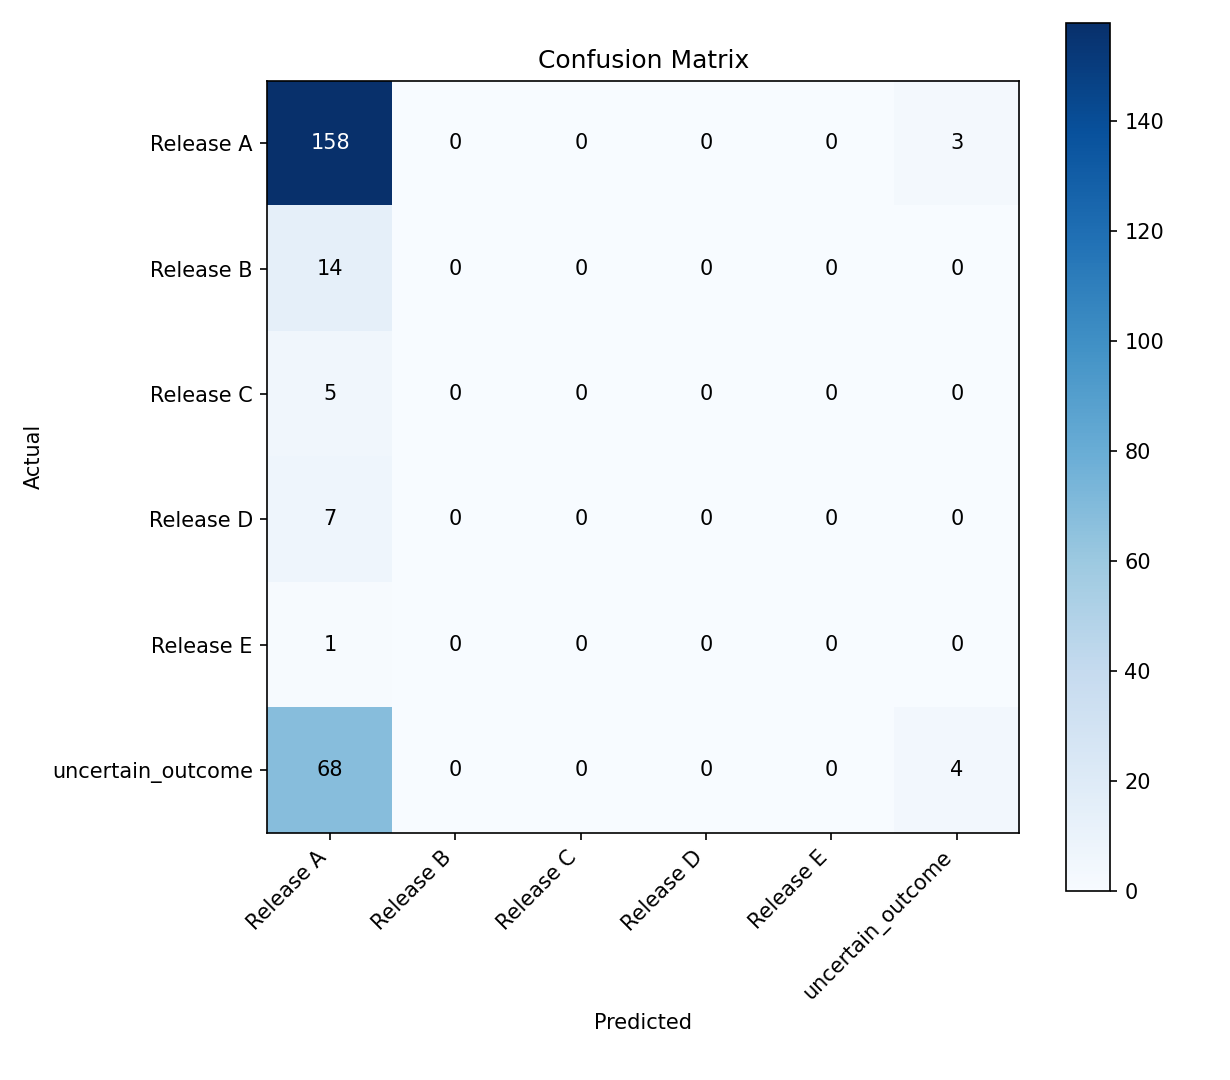
\includegraphics[width=0.48\textwidth]{figures/sepsis/alignments_confusion_matrix_len6.png}
	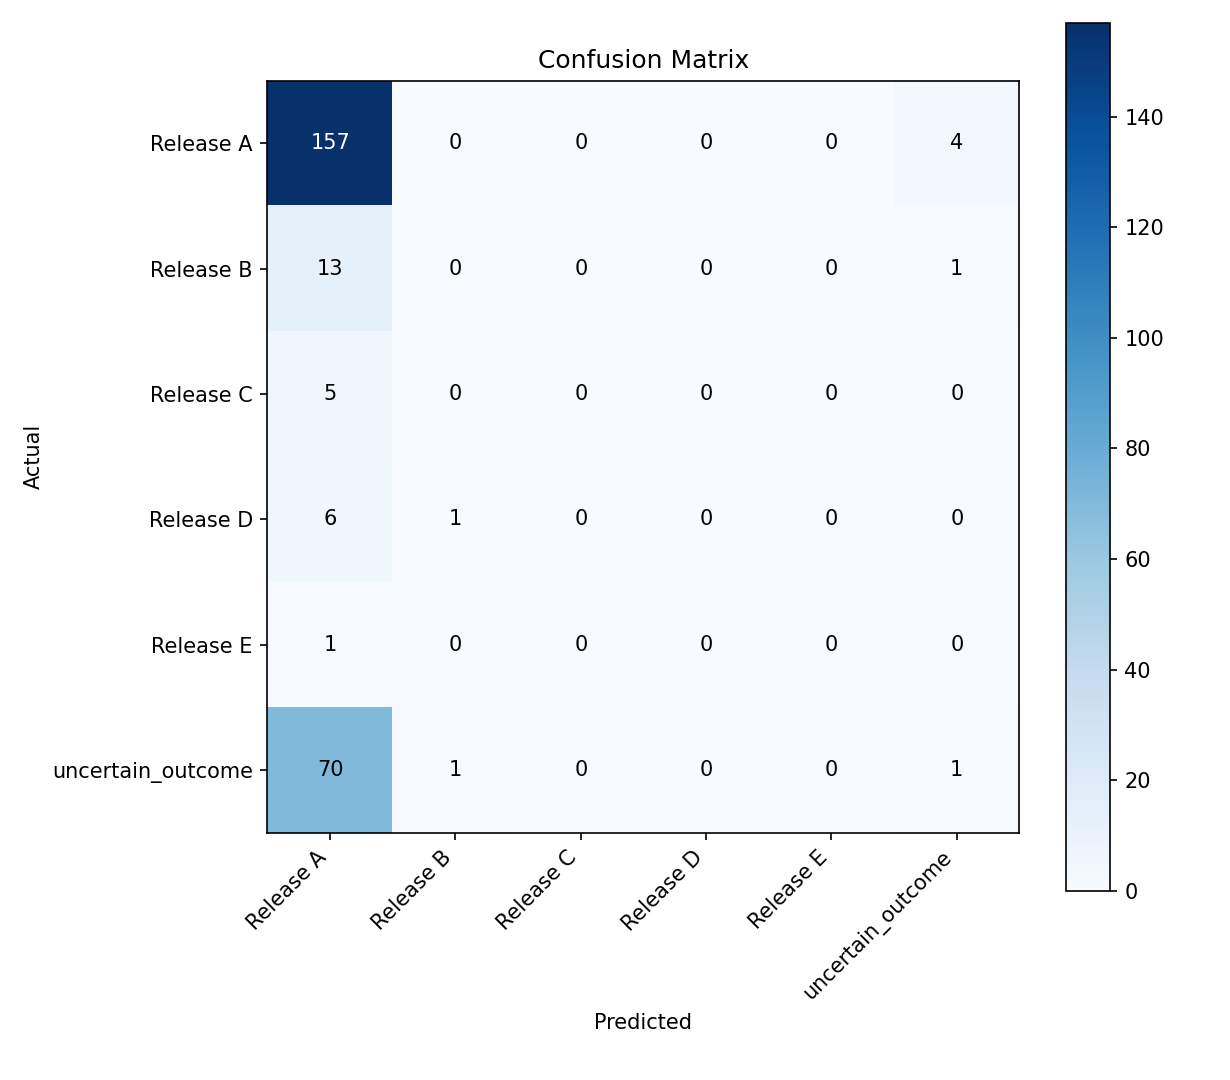
\includegraphics[width=0.48\textwidth]{figures/sepsis/alignments_confusion_matrix_len13.png}
	\caption{Confusion matrices for prefix length 6 (left) and 13 (right) for alignments classifier.}
	\label{fig:alignments_confusion_matrices}
\end{figure}
The alignment-based prediction approach has a very high recall of the majority label (\textit{Release A}) again, but poor class-accuracy for all other classes, including the uncertain outcome class. This can be seen in the confusion matrices \ref{fig:alignments_confusion_matrices} and the average class accuracy charts \ref{fig:alignments_per_class_accuracies}.
\begin{figure}[htbp]
	\centering
	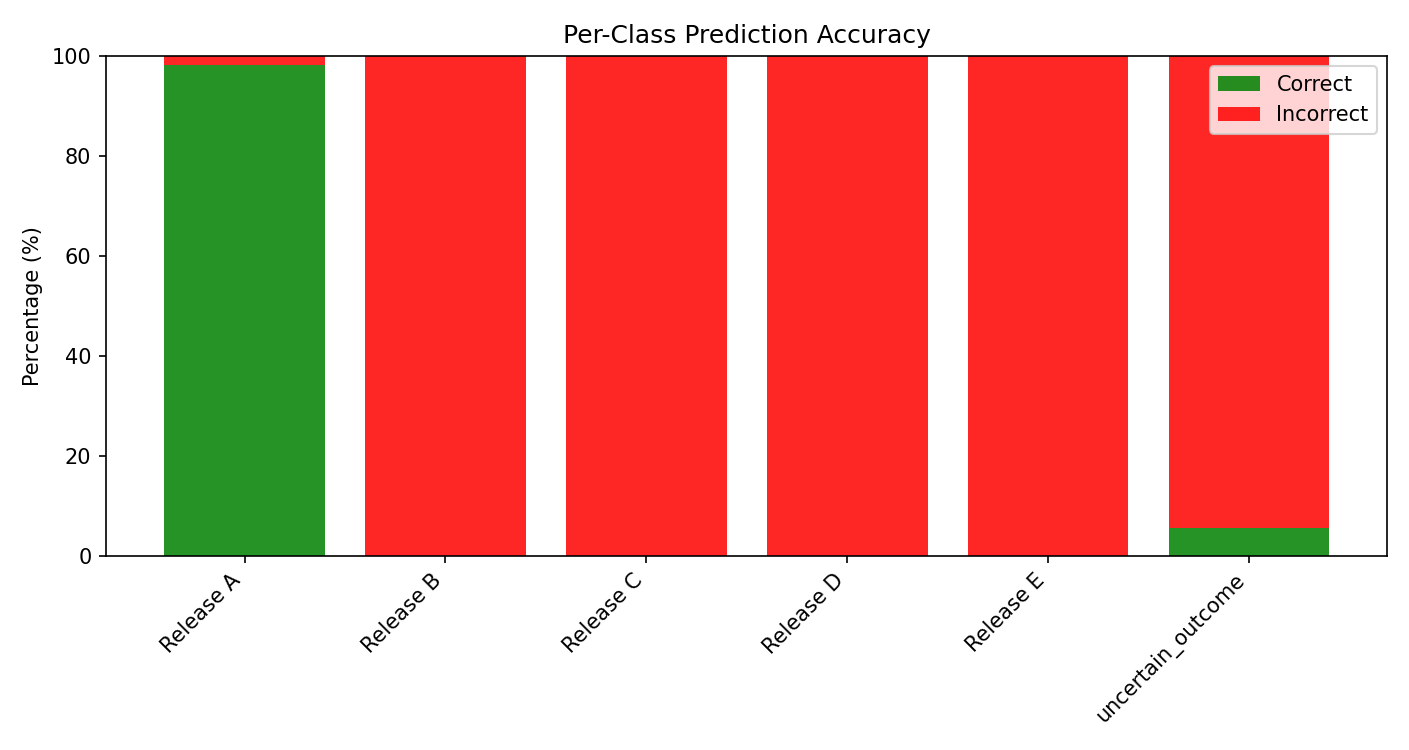
\includegraphics[width=0.48\textwidth]{figures/sepsis/alignments_per_class_accuracy_len6.png}
	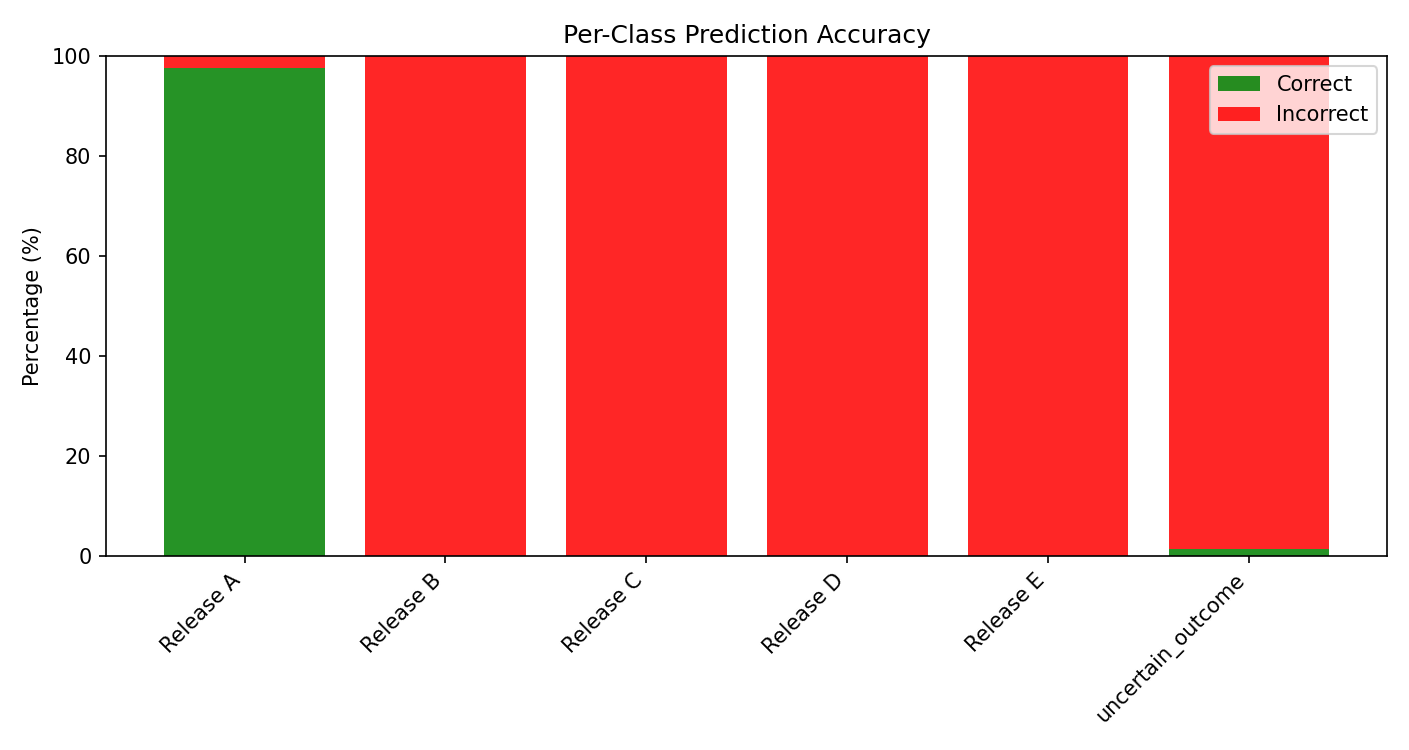
\includegraphics[width=0.48\textwidth]{figures/sepsis/alignments_per_class_accuracy_len13.png}
	\caption{Per-class accuracies for prefix length 6 (left) and 13 (right) for alignments classifier.}
	\label{fig:alignments_per_class_accuracies}
\end{figure}
Notably, an increase in prefix length did not improve the F1-score or the overall accuracy. This behavior is strange and hints at the classifier being overly biased toward the majority class due to the severe class imbalance, thereby failing to leverage the additional structural and behavioral deviation patterns captured by the alignments at longer prefix lengths.
\begin{figure}[t]
	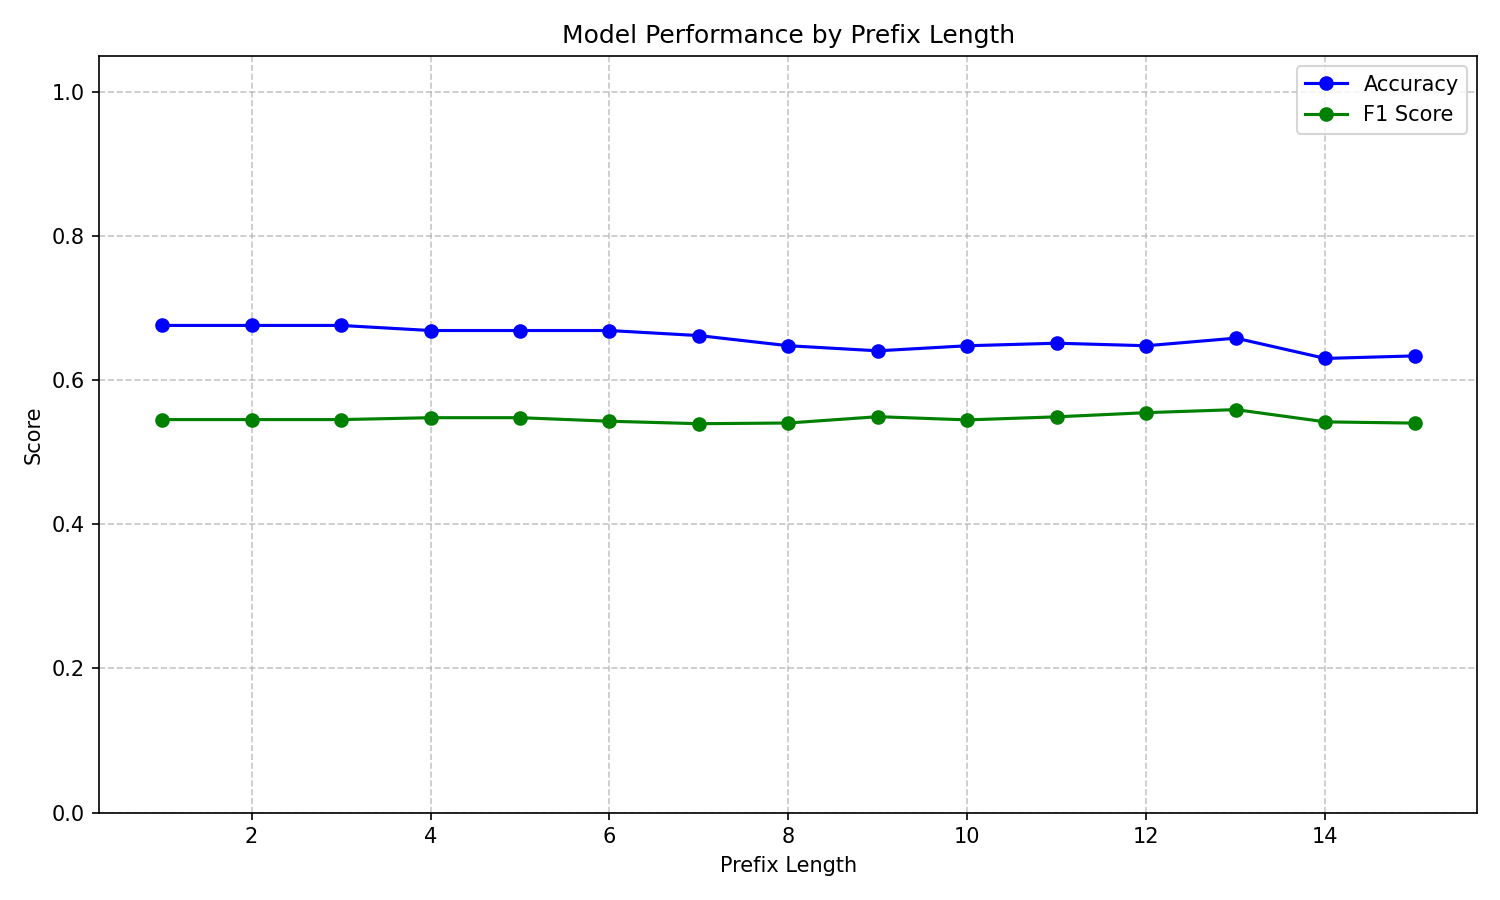
\includegraphics[width=1\textwidth]{figures/sepsis/alignments_by_len_vis.png}
	\caption{Accuracy and F1 score based on prefix length for alignments classifier.}
	\label{fig:alignments_by_len_vis}
\end{figure}

For the computational resource consumption we can clearly see, that aligning the train and test splits of the event log to the process model contributes mainly to the time the CLI pipeline took in total. Only about a third of the time was spent on tasks non-alignment related. The script's peak memory usage was about 259MB.
\begin{figure}[htbp]
	\centering
	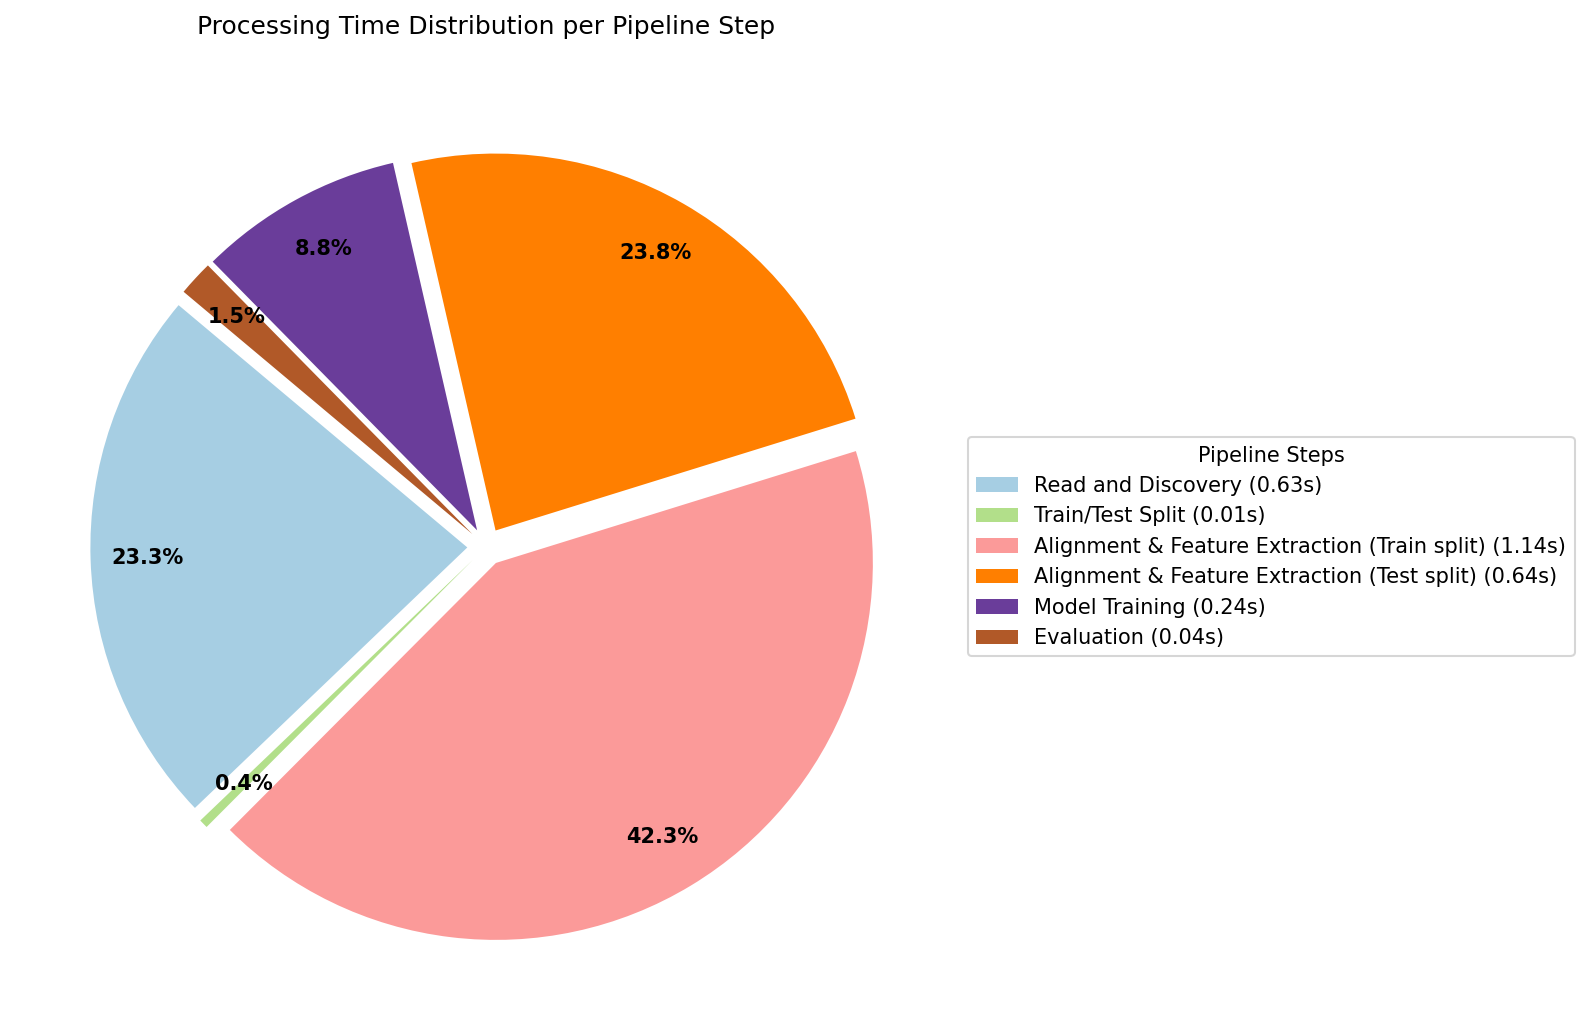
\includegraphics[width=1\textwidth]{figures/sepsis/alignments_runtime.png}
	\caption{Runtime of the alignments based classifier.}
	\label{fig:alignments_runtime}
\end{figure}

\subsection{Conclusion: Conformance-Aware vs. Conformance-Agnostic Predictive Monitoring}
In this experimental study, we evaluated the predictive capabilities of three distinct feature sets: control-flow (conformance-agnostic), static case attributes, and process alignments (conformance-aware) - to forecast process outcomes in the \textit{Sepsis Cases} event log.

The \textbf{conformance-agnostic approaches} (control-flow and case attributes) served as strong baselines. The case-attributes-only model immediately achieved a high baseline accuracy ($81\%$) due to the strong predictive power of static clinical indicators available at patient admission. Meanwhile, the control-flow-only model demonstrated a clear progression: as the prefix length increased from 1 to 15, the classifier gradually captured the sequential context of clinical interventions (e.g., \textit{IV Liquid}, \textit{Admission IC}), resulting in a steady performance climb (F1-score rising from $0.48$ to $0.78$). Both models, however, suffered significantly from the severe class imbalance, heavily favoring the majority outcomes (\textit{Release A} and \textit{uncertain\_outcome}).

In contrast, the \textbf{conformance-aware approach} utilizing alignment-based features presented a unexpected paradox. While alignments theoretically provide richer behavioral context by explicitly mapping actual traces against a normative process model, this approach did not yield the anticipated performance boost. Instead, the alignment-based classifier remained stagnated across varying prefix lengths. This behavior can be attributed to two main factors:
\begin{enumerate}
    \item \textbf{Model Generalization:} The normative model discovered by the Inductive Miner (noise threshold $0.2$) may have been too permissive or underfitting, leading to uniform alignment costs and features that failed to provide discriminative signals for minority classes.
    \item \textbf{Class Imbalance Vulnerability:} The structural deviation patterns captured by the alignments were entirely overshadowed by the overwhelming presence of the majority class, forcing the classifier to rely on majority-label shortcuts.
\end{enumerate}

Furthermore, from a resource consumption perspective, the conformance-aware pipeline introduces a severe bottleneck. While conformance-agnostic feature extraction is computationally lightweight and scales linearly, alignment computation scales exponentially with trace prefix lengths, drastically increasing peak memory and runtime without delivering a proportional dividend in accuracy or F1-score.
For highly imbalanced healthcare process logs like \textit{Sepsis Cases}, a conformance-agnostic approach combining static case attributes with early control-flow prefixes yields the most efficient and accurate predictive performance. Conformance-aware (alignment-based) predictive monitoring should only be deployed if the underlying process model is strictly constrained, highly reliable, and where identifying structural deviations is a primary, explicit domain requirement rather than a proxy for outcome classification.

\begin{thebibliography}{10}
\bibitem{feature_importance}
Michael Allen, \textit{Random Forest and SHAP Values}, 2022.
\url{https://michaelallen1966.github.io/titanic/27_random_forest_shap.html} (visited June 2026).
\bibitem{sepsis_study}
Mannhardt, F., \& Blinde, D., \textit{Analyzing the trajectories of patients with sepsis using process mining}, 2017.
\url{https://pure.tue.nl/ws/portalfiles/portal/68704626/bpmds_08_paper.pdf}
\end{thebibliography}

\end{document}
